\section{Auswertung}
\label{sec:Auswertung}

Die Formel für den Mittelwert lautet
 \begin{equation}
    \bar{x}=\frac{1}{n}\sum_{i=1}^n x_i .
\end{equation}

Die Formel für die Standardabweichung lautet
\begin{equation}
    s_x=\sqrt{\frac{1}{n-1}\sum_{i=1}^n {(x_i-\bar{x})^2 }}.
\end{equation}

Die Formel für den Fehler des Mittelwertes lautet
\begin{equation}
    \Delta \bar{x} = s_{\bar{x}}=\frac{s_x}{\sqrt{n}}= \sqrt{\frac{1}{n(n-1)}\sum_{i=1}^n {(x_i-\bar{x})^2 }}.
\end{equation}

Die Formel für den Fehler des Mittelwertes lautet
\begin{equation}
    \Delta \bar{x} = s_{\bar{x}}=\frac{s_x}{\sqrt{n}}= \sqrt{\frac{1}{n(n-1)}\sum_{i=1}^n {(x_i-\bar{x})^2 }}.
\end{equation}

$V$

In Tabelle 1 sind die gemessenen Werte aufgeführt und die Ausgleichskurve ist in Abbildung 1 dargestellt.
\begin{table}
  \centering
  \caption{Messdaten.}
  \label{tab:some_data}
  \begin{tabular}{ccc}
    \toprule
    $N_{Linie}$ & $D /   \mathrm{mm}$  & $U /  \mathrm{V} $\\
    \midrule
    1 & 0 & -19,5 \\
    2 & 6 & -16,1 \\
    3 & 12 & -12,4 \\
    4 & 16 & -9,6\\
    5 & 24 & -6,2 \\
    6 & 30 & -2,4 \\
    7 & 36 & 1,2 \\
    8 & 42 & 5,1 \\
    9 & 48 & 8,3 \\

    \bottomrule
  \end{tabular}
\end{table}

Die Abstände werden umgerechnet durch die Formel
\begin{equation}
  D = (N_{Linie}-1) \cdot 6  \mathrm{mm}.
\end{equation}

\begin{align*}
  m &= (1,7193 \pm 0,0197)  \si{\milli\meter\per\volt}    \\
  b &= (33,8571 \pm 0,2102 )  \si{\milli\meter} .\\
\end{align*}


\begin{figure}
  \centering
  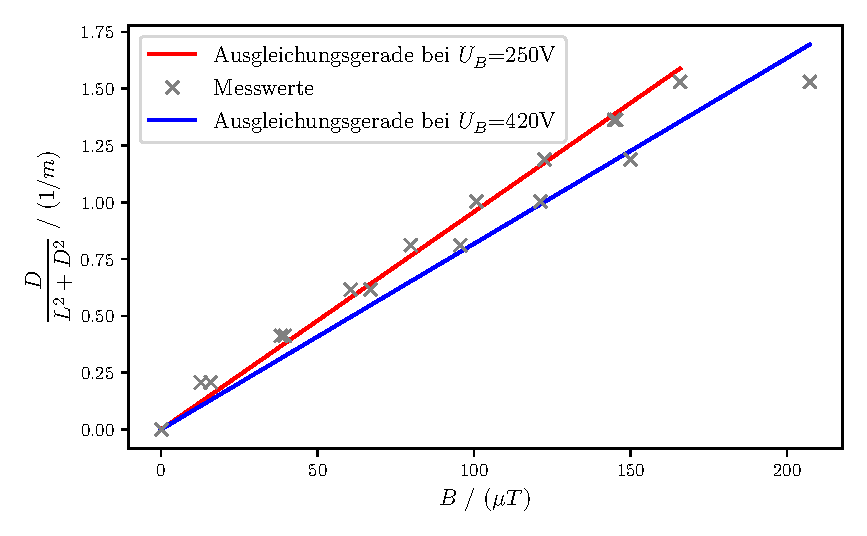
\includegraphics{plot.pdf}
  \caption{Plot.}
  \label{fig:plot}
\end{figure}


Siehe \autoref{fig:plot}!
